\section{Рабочий проект}

\subsection{Классы, используемые при разработке приложения}

В процессе разработки программной реализации продукционной системы Маркова была создана архитектура, основанная на использовании нескольких ключевых классов. Каждый класс выполняет строго определённую роль в обработке входных данных, применении правил, формировании журнала шагов и вычислении статистических показателей.

Основные классы Python, применяемые при реализации системы, приведены в таблице \ref{class:markov}.

\renewcommand{\arraystretch}{0.8}
\begin{xltabular}{\textwidth}{|X|p{3cm}|X|X|}
	\caption{Описание классов Python, используемых в приложении \label{class:markov}}\\
	\hline \centrow Название класса & \centrow Модуль & \centrow Описание & \centrow Основные методы \\ \hline
	\endfirsthead
	\caption*{Продолжение таблицы \ref{class:markov}}\\
	\hline \centrow Название класса & \centrow Модуль & \centrow Описание & \centrow Основные методы \\ \hline
	\finishhead
	
	MarkovRules & core &
	Класс, отвечающий за хранение структуры отдельного правила (левая и правая части), обработку признака остановки и применение правила к тексту. &
	\texttt{apply(text)} — применяет правило к строке; возвращает новую строку и флаг остановки. \\ \hline
	
	MarkovSystem & core &
	Основной класс, реализующий цикл работы системы Маркова. Обеспечивает последовательное применение правил, ведение журнала шагов и расчёт статистики. &
	\texttt{run(text)} — выполнение системы; \texttt{save\_log(log)} — сохранение журнала;
	\texttt{show\_stats()} — вывод статистических данных. \\ \hline
	
	LogManager & utils &
	Модуль для управления журналом шагов, хранения промежуточных состояний строки и передачи данных в визуальный модуль. &
	\texttt{add(entry)} — добавляет новую запись;
	\texttt{export(path)} — сохраняет журнал в файл. \\ \hline
	
	GUIController & ui &
	Класс, отвечающий за работу графического интерфейса, обработку событий пользователя, пошаговую визуализацию и отображение текущей статистики. &
	\texttt{start()} — запуск интерфейса;
	\texttt{animate()} — анимация применения правил;
	\texttt{update\_stats()} — обновление панели статистики. \\ \hline
\end{xltabular}
\renewcommand{\arraystretch}{1.0}

\subsection{Модульное тестирование}

Для проверки корректности работы отдельных компонентов системы было проведено модульное тестирование. Тесты охватывают работу правил, корректность остановки, поведение системы при отсутствии совпадений, а также обработку ошибочных входных данных.

Пример теста метода \texttt{apply} класса \texttt{MarkovRules} представлен ниже:

\begin{lstlisting}[language=Python]
	def test_apply_rule():
	rule = MarkovRules("ab", "c")
	text, stop = rule.apply("abcab")
	assert text == "ccab"
	assert stop == False
\end{lstlisting}

Этот тест демонстрирует базовую проверку правильности применения правила: проверяется количество замен, корректность итоговой строки и отсутствие преждевременной остановки.

Дополнительные тесты включают:
\begin{itemize}
	\item проверку обработки правил с точкой (остановка системы);
	\item применение правил без совпадений (строка остаётся неизменной);
	\item корректность приоритетного выбора верхнего правила;
	\item работу цикла системы при различных наборах правил.
\end{itemize}

\subsection{Системное тестирование}

Системное тестирование охватывает проверку всей цепочки преобразований, включая загрузку правил, обработку строки, генерацию журнала шагов и вывод статистических данных.

Ниже приведён пример работы программы в консольном режиме:

\begin{verbatim}
	$ python markov_system.py
	Введите исходную строку: ababc
	Правила загружены: ab -> c, a -> x.
	Шаг 1: ababc -> ccabc  | правило: ab -> c
	Шаг 2: ccabc -> ccxbc  | правило: a -> x
	...
	Результат: ccxbc
	Всего шагов: 2
	Средняя длина строки: 5.0
	Самое частое правило: ab -> c (1 раз)
	Журнал шагов сохранён в log.txt
\end{verbatim}

Системное тестирование также включало проверку:
\begin{itemize}
	\item обработки больших строк (до 50\,000 символов);
	\item применения более сотни правил;
	\item корректного поведения при рекурсивных заменах;
	\item устойчивости интерфейса при длительной анимации.
\end{itemize}

\subsection{Графический интерфейс и анимация работы алгоритма}

Для визуализации работы алгоритма была разработана графическая оболочка на основе библиотеки \texttt{customtkinter}. Интерфейс включает следующие элементы:

\begin{itemize}
	\item поле ввода исходной строки;
	\item окно просмотра списка правил;
	\item форму для добавления новых правил вручную;
	\item кнопку запуска системы;
	\item панель отображения текущего шага преобразования;
	\item анимацию замены подстрок в реальном времени (подсветка найденных фрагментов).
\end{itemize}

Пример окна интерфейса показан на рисунке~\ref{gui_main_window}.

\begin{figure}[h!]
	\centering
	\fbox{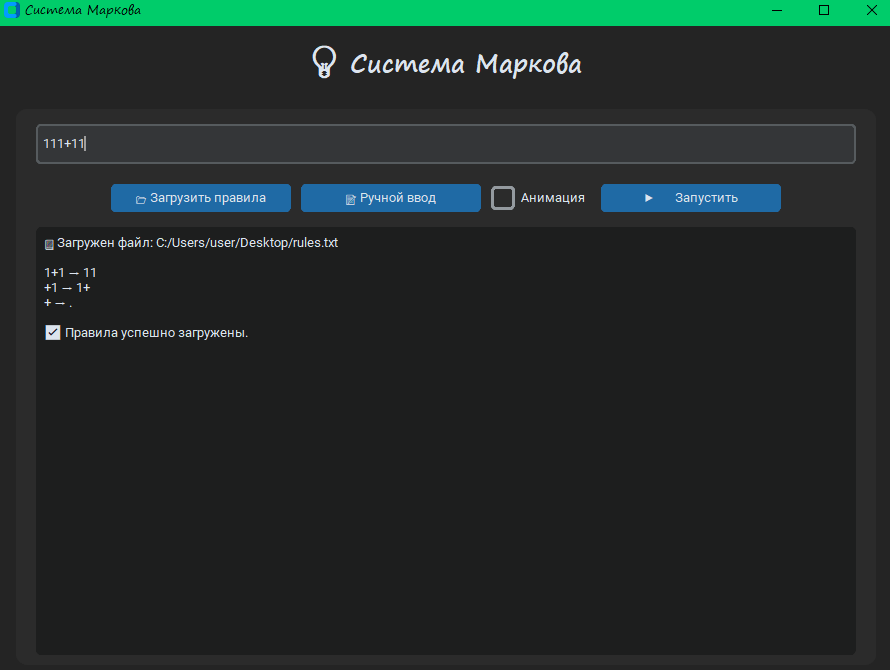
\includegraphics[width=0.9\textwidth]{images/gui_main.png}}
	\caption{Главное окно графического интерфейса приложения}
	\label{gui_main_window}
\end{figure}

Анимация показывает:
\begin{itemize}
	\item выделение найденного фрагмента цветом;
	\item плавную замену текста;
	\item обновление счётчика шагов;
	\item в реальном времени — текущую длину строки.
\end{itemize}

На рисунке~\ref{gui_animation} приведён пример работы анимации.

\begin{figure}[h!]
	\centering
	\fbox{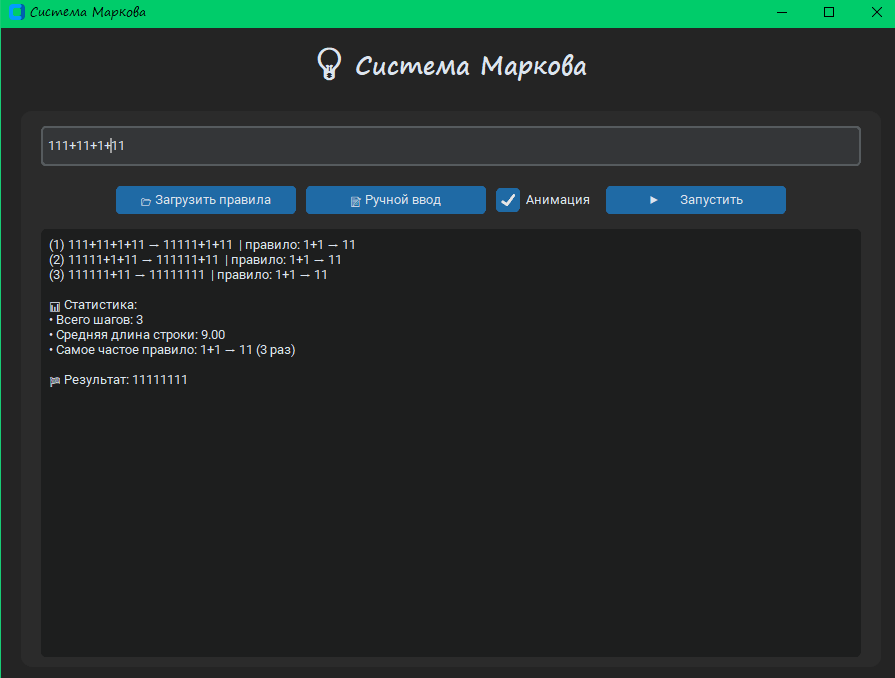
\includegraphics[width=0.9\textwidth]{images/gui_animation.png}}
	\caption{Пошаговая анимация работы правила}
	\label{gui_animation}
\end{figure}

\subsection{Отображение статистики и журнала шагов}

В приложении предусмотрен отдельный экран для визуализации статистики работы системы. Он включает:

\begin{itemize}
	\item общее количество выполненных шагов;
	\item наиболее часто применяемое правило;
	\item среднюю длину строки;
	\item график изменения длины строки по шагам;
	\item таблицу всех применённых правил.
\end{itemize}

На рисунке~\ref{stats_window} показан пример окна статистики.

\begin{figure}[h!]
	\centering
	\fbox{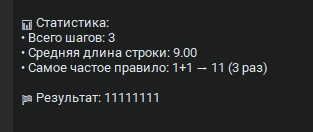
\includegraphics[width=0.9\textwidth]{images/stats_window.png}}
	\caption{Окно статистики работы системы Маркова}
	\label{stats_window}
\end{figure}

Также реализован режим просмотра журнала шагов. Пользователь может перелистывать шаги, анализировать изменения строки и сохранять журнал в файл.

\begin{figure}[h!]
	\centering
	\fbox{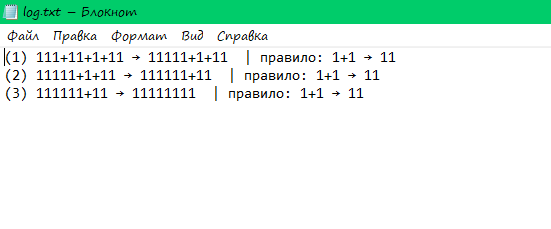
\includegraphics[width=0.9\textwidth]{images/log_window.png}}
	\caption{Просмотр журнала шагов работы системы}
	\label{log_window}
\end{figure}

\subsection{Особенности реализации}

Основные особенности разработанного приложения включают:

\begin{itemize}
	\item поддержку правил с точкой (остановка работы после применения правила);
	\item ведение расширенной статистики (медианная длина, дисперсия, количество замен каждым правилом);
	\item сохранение журнала шагов в форматах TXT и JSON;
	\item возможность пошагового выполнения с анимацией или мгновенной симуляции;
	\item устойчивость интерфейса при длительных вычислениях;
	\item поддержку загрузки правил из файлов формата \texttt{.mrk}.
\end{itemize}


Таким образом, разработанное приложение представляет собой полноценную продукционную систему Маркова, включающую как консольный интерфейс, так и графическую оболочку с анимацией и визуальной статистикой. Программа может использоваться как учебное средство для изучения формальных моделей вычислений и как инструмент анализа свойств строковых систем.